\subsection{System Overview}
\label{subsec:methodology-system-overview}

This work presents a control framework for quadruped robots capable of generating dynamic, acyclic gaits in challenging environments. The framework employs a hierarchical architecture that processes robot state and terrain data to produce footstep commands for the robot controller. 

The first stage of the framework receives user input $\mathbf{v^{usr}}$ alongside the tracking robot state $\mathbf{x_g}$ into the gait generation network (\textit{GaitNet}). GaitNet acts as an evaluative surface, performing continuous optimization over the physical workspace using projected gradient ascent. Rather than extracting from a discrete sample grid, GaitNet iteratively ranks these continuous spatial variables to yield an optimal footstep action $\mathbf{f_a}$. This optimal action is then passed downstream to a traditional MIT Mini-Cheetah Controller \cite{di_mini_cheetah_2020}. This hierarchical design ensures strict control over potential actions and prevents violations of physical constraints.

\begin{figure}[H]
  \centering
  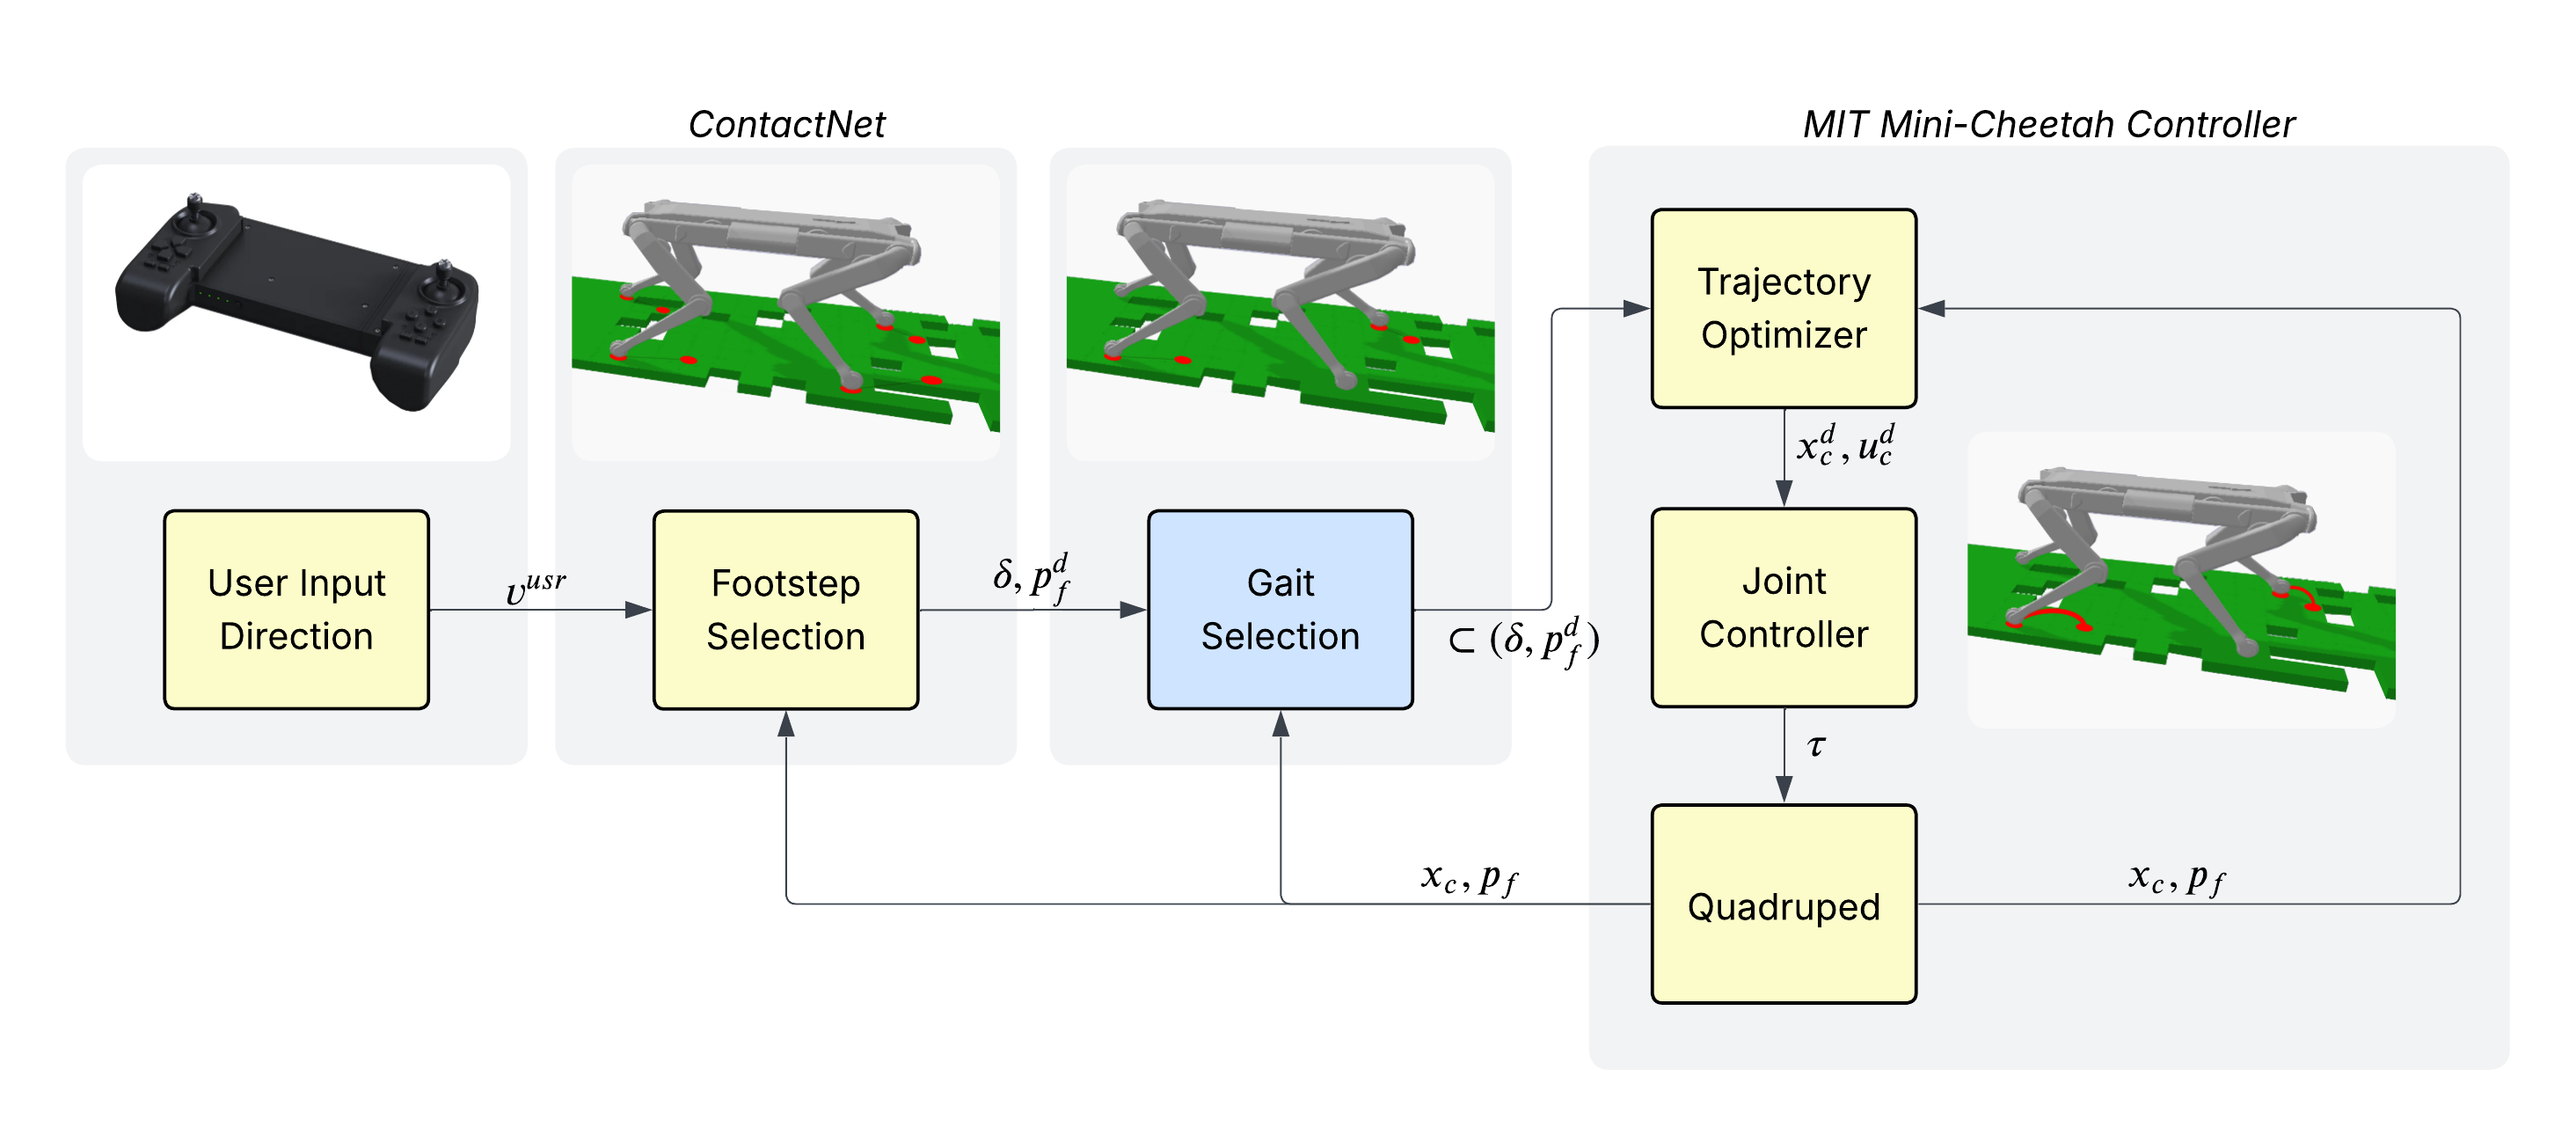
\includegraphics[width=0.7\linewidth]{images/diagrams/control-system.png}
  \caption{Block diagram of the proposed framework. The user defines an input direction $\mathbf{v^{usr}}$, which GaitNet uses along with the robot state $\mathbf{x_g}$ and current foot positions $\mathbf{p_f}$ to evaluate candidate footsteps. GaitNet utilizes a continuous projected gradient ascent optimization strategy to generate optimal step actions $\mathbf{f_a}$ for the controller.}
  \label{fig:diagram-control-system}
\end{figure}

\subsection{GaitNet Architecture}
\label{subsec:methodology-gaitnet-architecture}

GaitNet is a single-network architecture composed of a state encoder, footstep encoder, shared trunk, and two task-specific output heads (one predicting logit rewards and another predicting swing duration). It ranks footstep candidates based on the one-hot encoded leg index $\mathbf{f_c}^{\prime}$ and the state $\mathbf{x_g}$, which tracks the current base position $\mathbf{p}_{b,xy}$ and rotation $\mathbf{r}_{w,z}$, body velocities $\mathbf{v}_b$ and $\mathbf{\omega}_b$, current foot positions $\mathbf{u}$, gravity $\mathbf{g}$, and contact state $\mathbf{c}$. Both the continuous spatial coordinates and a fixed ``no-action'' embedding are evaluated simultaneously.

\subsection{Projected Gradient Ascent Optimization}
\label{subsec:methodology-gaitnet-gradient-ascent}

Footstep selection is formulated as a continuous optimization problem over the spatial coordinates. GaitNet’s predicted reward logit acts as a differentiable objective function maximized via projected gradient ascent.

For each foot, $N=4$ random initial spatial samples are drawn uniformly from the reachable kinodynamic workspace. The algorithm performs 4 parallel steps of projected gradient ascent to maximize the GaitNet evaluation logit. After each gradient update step, spatial coordinates are projected back to the nearest valid configuration within the reachable stepping continuous space (c-space). This projection acts as a hard constraint that forces foot locations to avoid un-steppable obstacles (such as gaps or rough geometry) while preserving maximal reward.

Concurrently, a fixed ``no-action'' embedding is evaluated. Once the 4 projection and ascent steps finish, the candidate yielding the highest reward logit across all $4 \times 4$ tracks is compared to the ``no-action'' logit. The action with the maximum reward is output as $\mathbf{f_a}$ and deployed to the inner controller at control frequencies.

\subsection{Network Training}
\label{subsec:methodology-gaitnet-training}

GaitNet is trained using Proximal Policy Optimization (PPO) \cite{Schulman_proximal_2017} acting directly as the policy network, with a structurally similar critic network. Given the dual discrete-continuous nature of the task, the logits parameterized a categorical distribution over tracks, while the duration output constitutes a normal distribution with fixed standard deviation. The continuous spatial coordinates are trained synchronously under the PPO agent formulation.
